%% -*- coding: utf-8-unix -*-

% \begin{lstlisting}[caption=,label=lst:]
% \end{lstlisting}

\chapter{テストシナリオ実装}
\label{chap:poc-scenario-dev}

PoCで実施したテストシナリオの実装、実際にテスト自動化をおこなってわかっ
たことや注意事項などについて解説する。

 \section{テストシナリオの概要}

  \subsection{ネットワークテストの方針}

\ref{chap:poc-target-design}章で設定したとおり、\yo ネットワークのテスト
を考える。そのためのテストシナリオとして「静的なふるまいのテスト」「動的
なふるまいのテスト」の2種類を実装する。テストシナリオ実装・テスト実行を
通して、物理ネットワークのテストを自動実行する際のポイントや問題点の抽出、
従来の人手によるテスト作業との比較をおこなう。

  \subsection{BDDテストシナリオの基礎}
  % - TDD/BDDとBDDツールとしてのCucumber
  % - Narrative
  % - ネットワークテストを書く上での検討点、今回のプロジェクトでの方針・決めごと
  %   - なぜそうきめたのか?

      \paragraph{テストツール}
NetTesterはテスト用ノードの生成・テスト対象ネットワークへの配置(パッチ接
続)をおこなうためのAPIを提供する。提供されるAPIを使用して \yo ネットワー
クのテストを実装する。\footnote{実際に作成した自動テストのためのコードは
NetTester Examples~\cite{nettester-ex}として公開している。}

テストシナリオの記述については、アプリケーションのテストでつかわれる既存
のツールと連携することを想定している。本PoCでは、
\begin{itemize}
 \item 「BDDによるネットワークのテスト」を考えていること
       (\ref{sec:behavior-test}節)
 \item 広く使われているツールであること
 \item RubyベースでNetTesterとの親和性が高いこと
\end{itemize}
をもとに、BDDツールであるCucumber\cite{cucumber}を採用した。

    \paragraph{Narrative}
    % Cucumber の .feature の書き方 – NetTester
    %   https://3.basecamp.com/3088280/buckets/867009/messages/155991347
    % クライアントの要望にこたえるWebサービス開発 ~「らせん型ワークフロー」のススメ~
    %  http://www.slideshare.net/mayuco/css-nite-in-sapporo-vol5-14085124
BDDでは、テストのストーリー(フィーチャ)を以下のような構造で記述する
\cite{rspec-book,spiral-workflow}。
\begin{description}
 \item[タイトル] どのストーリーについて説明するのかを示す。タイトルは一
            般に、ユーザがシステムに要求するかもしれないアクティビティを
            短い言葉で表したものになる。
 \item[ナラティブ] ストーリーの内容について説明をする。一般的には
            Connextraフォーマットと呼ばれる形式の短い文章で記述される。
            このテンプレートは、誰がシステムを使っていて・そのユーザは何
            をしていて・なぜそのことに関心があるのか、を明確にする。
            \begin{itemize}
             \item ``As a (role)'': [誰のために(role)]として
             \item ``I want (feature)'': [何を(feature)]したい
             \item ``So that (bussiness value)'': なぜなら[なぜ
                   (bussiness value)]のためだ
            \end{itemize}
 \item[受け入れ基準] ストーリーの完了・完成を定義する受け入れ基準、シナ
            リオの定義。
\end{description}

Cucumberにおけるフィーチャとは、システムを利用するユーザーの視点に立って
おおまかに表現された要件のことを指す。Cucumberのフィーチャはタイトルと簡
単なナラティブ、受け入れ基準としての役割をはたす自動化されたシナリオによっ
て構成される。
\begin{itemize}
 \item フィーチャはタイトルとナラティブで構成され複数のシナリオを含む。
       (本プロジェクトでは\verb|features/*.feature|ファイル)
       \begin{itemize}
        \item シナリオはそれぞれ、シナリオ内でおこることを任意のステップ
              で記述する。
       \end{itemize}
 \item 個々のステップ定義は開発で使っているシステムの言語で記述される。
       (本プロジェクトではRuby: \verb|features/step_definitions/*.rb|ファ
       イル)
\end{itemize}

% Narrative を Pull Requst する – NetTester
%   https://3.basecamp.com/3088280/buckets/867009/todos/159223633
% NetTester機能拡張(NW機器間接続)方針・やりたいこと – NetTester
%   https://3.basecamp.com/3088280/buckets/867009/todos/182746431
% Firewall の cucumber シナリオ – NetTester
%   https://3.basecamp.com/3088280/buckets/867009/todos/158299550

 \section{静的なふるまいのテスト}
% テストシナリオ策定の考えかた…そもそもなにをするテストなのか。どのような
% 検討を経てテストシナリオをきめたのか。narrativeの定義のプロセスとか。
% TODO: OOD資料にかいたようなテストコード解説のはなしをこちらにも含めるか?
% - 実装
%   - Step2テスト業務で気づいたことをまとめる – NetTester
%     \url{https://3.basecamp.com/3088280/buckets/867009/todos/260220903}

  \subsection{テストとして実現したいこと}
ネットワークに対して最低限要求されることは、ネットワークを介して必要な通
信が実現できることである。ネットワークの目的は、大きく言えばコミュニケー
ションを実現することである。あるノードが、他のノードと、必要な手段(アプ
リケーション)で通信できるかどうか、という点がまず初めにネットワークに求
められる機能要求となる。

「ネットワークの静的なふるまい」(\ref{sec:behavior-to-test}節)では、ネッ
トワークが定常状態にあるときに、ネットワーク利用者が実現したいend-to-end
の通信がすべて実現可能かどうかをテストする。

  \subsection{テスターに求められる機能}

テストで確認したいend-to-endの通信、すなわち、実現したい通信要求は、通信
をおこなうノード(エンドポイント)の論理的・物理的な配置の組合せに応じて異
なる。また、通信をおこなうアプリケーションによっても別途制御がおこなわれ
る。例えば、DPIをおこなうFWやLBなどがネットワーク内にある場合は、単純な
宛先(ヘッダ)情報だけではなく、やりとりされるアプリケーションレベルの情報
によって通信の可否などが変化する。

したがって、単純なend-to-endの通信試験だとしても、
\begin{itemize}
 \item 配置やアプリケーションの組合せによって大量のテストケースが発生し
       てしまう
 \item テスト用のリソース(端末や人など)確保が充分にできない
\end{itemize}
などの課題があった(\ref{sec:discuss-network-test}節)。

そこで、テスター(NetTester)では以下の機能が要求される。
\begin{itemize}
 \item テスト用ノードの生成
 \item テスト用ノードの配置
 \item テスト用ノード上でのタスク実行
 \item 複数のテスト用ノード操作/集中管理
\end{itemize}
NetTesterはこうしたノードの生成・配置・集中制御の機能(API)を提供している。
テストシナリオ(Cucumber)ではBDDの考えかたに基づいて、ノード間でどういっ
た通信を実現する必要があるかを個別の通信要件
(\ref{sec:network-requirements}節)ごとに定義する。

  \subsection{静的なふるまいのテストで実際に発見できた問題点}
  \label{sec:statictest-founded-issues}

静的なふるまいのテストでは、\yo ネットワーク通信要件
(\ref{sec:network-requirements}節)それぞれについてテストシナリオを実装し、
個々の要件に対してend-to-endの通信試験が自動化できることを実証した。テス
トの実行によって実際に発見できた物理ネットワークの問題点について解説する。

   \subsubsection{テスト対象ネットワークの設定不備の発見}
 % DNSのテスト作る – NetTester
 % https://3.basecamp.com/3088280/buckets/867009/todos/301325453
 % 通信要件\#29 B社PC→DMZ内のVPNサーバの疎通確認(SSLVPN) – NetTester
 % https://3.basecamp.com/3088280/buckets/867009/todos/233178490

 % 通信要件\#10 A社内PC→インターネットの疎通確認(ICMP) – NetTester
 % https://3.basecamp.com/3088280/buckets/867009/todos/233175867
 % 通信要件#27インターネット→ファイアウォールの疎通確認(ICMP) – NetTester
 % https://3.basecamp.com/3088280/buckets/867009/todos/233178319

一般的な(人手による)疎通試験と同様に、pingやその他のアプリケーションによ
る通信確認によって、テスト対象ネットワーク上の不備(要求される仕様と異な
る)点あるいはそれにつながる事象を発見できた。

    \paragraph{テスト対象ネットワークの設定ミス}
テスト対象ネットワークを構築した際の設定ミスによる問題を発見した。主要な
ものはFWパケットフィルタルールの設定不備、NAT(NAPT)の設定ミスによるもの
である。これらは「できなければいけないこと」ができていない(テストが失敗
する)ことによって発見されたものである。以下に例を示す。
\begin{itemize}
 \item インターネットからNAT(VIP)を経由してDMZへアクセスする通信失敗(パ
       ケットフィルタルールの設定漏れ)
 \item \yo 内部ゾーンから外部ゾーン(internet)への通信失敗(NAPT設定ミス)
 \item FWが持つIPに対するping失敗(FWデフォルトのping応答ポリシ設定漏れ)
\end{itemize}

    \paragraph{テスト作業者側(構築・運用側)の通信仕様の認識違い}
登場人物(\ref{sec:poc-casting}節)に示したように、テストシナリオの実装や
実行をおこなった担当者は必ずしもネットワークやネットワーク機器のスペシャ
リストではない。そのため、FWゾーン間通信ルールについての認識不足
\footnote{ゾーン間通信のデフォルトポリシについて、当該機器を使用したこと
があるネットワークエンジニアとしては自明だったために明確に伝達がおこなわ
れていなかった。}から、\yo 外部ゾーン(インターネット)から内部ゾーンへの
ping通信が可能と判断してテストシナリオを実装してしまったケースがあった。
実際には要件どおり設定されたFWによってこのテストが失敗し、認識違いがあっ
たことが判明した。

   \subsubsection{ネットワーク機器の動作不具合}
   \label{sec:find-nw-device-bug}
 % 原因切り分けメモ (muraki) – NetTester
 % https://3.basecamp.com/3088280/buckets/867009/documents/217782147
 % 調査: テスト環境でシナリオ実行すると2回目以降でコケる – NetTester
 % https://3.basecamp.com/3088280/buckets/867009/todos/218486066

当初、静的なふるまいのテストを実装し、動作させたときに、同一のテストシナ
リオが実行されるたびに成功・失敗をくりかえすという事象があった。FWの動作
を調査したところ、ARP処理の挙動について以下のような動作をしていることが
わかった。
\begin{itemize}
 \item NetTesterが生成するテスト用ノードでは、IPアドレスは一定だが、MAC
       アドレスはテストシナリオ実行ごとにランダムに変更する。
 \item FWにARP前のシナリオで実行したテスト用ノードのMACエントリが残って
       いると、次のシナリオで実行した(IPは同一だがMACアドレスが異なる)ARPに
       対して応答しない。(ARPエントリのクリアをおこなっても応答しない。)
 \item FWのARPエントリをクリアして、クライアントからTCP通信をおこなって
       もFW(Gateway)からサーバへのARPが確認できない。また、MACアドレスを
       学習していないにもかかわらず TCP SYN が送信されることがある。
\end{itemize}

これらの事象および当初使用していたFWのOSバージョンが古かったことから、
FW(OS)の不具合と判断し、FWのOSを更新する
\footnote{\tabref{tbl:device-list}参照。FWは更新版6.3.0r22.0(2016/4月リ
リース)に対して当初は6.3.0r5.0(2010/9月リリース)を使用していた
\cite{screenos-releases}。}ことで解決した。

   \subsubsection{L7レベルのFW挙動変化}
今回のテストシナリオ実装では、当初L4レベルの通信確認から実装し、可能なも
のについては実際のサーバ/クライアントを使用したL7レベルでの実装をおこなっ
ている。L4レベルの通信確認としては、netcat を使った任意の TCP/UDP port
listenとクライアントからの接続(tcpセッション確立/単純なサーバからの応答
確認)を使用している。L7レベルのend-to-endテスト実装としては以下のシナリ
オがある。
\begin{itemize}
 \item インターネットへのSSLアクセス(openssl/WEBrick, curlを使用したテス
       トシナリオ実装
       \footnote{\url{https://github.com/net-tester/examples/blob/feature/ood_demo/features/step_definitions/google_steps.rb}}, \ref{sec:test-client-exec}節)
 \item SSHサーバヘのアクセス(opensshを使用したテストシナリオ実装
       \footnote{\url{https://github.com/net-tester/examples/blob/feature/ood_demo/features/step_definitions/ssh_steps.rb}})
 \item DNSサーバへのアクセス(dnsmasqを使用したテストシナリオ実装
       \footnote{\url{https://github.com/net-tester/examples/blob/feature/ood_demo/features/step_definitions/dns_steps.rb}})
\end{itemize}

特に、DNSのテストについては、当初 netcat によるL4レベル確認として実装し
たが、テストが成功しなかった(FWを経由して通信ができなかった)。このとき
\code{dig}コマンド等による実際の名前解決はできていたことから、テストシナ
リオとしてもdnsmasqによるL7レベルでのトラフィック生成シナリオを実装して
いる。

 \section{動的なふるまいのテスト}
% 障害試験シナリオを書く – NetTester
% \url{https://3.basecamp.com/3088280/buckets/867009/todos/238169066}
% Step2to3タスク検討
% https://drive.google.com/open?id=0B2eRR_JxYJA5M1RGdEZaOFkxTFk

  \subsection{テストとして実現したいこと}
  \label{sec:dynamic-test-target}
% NetTester機能拡張検討
% https://drive.google.com/file/d/0B2eRR_JxYJA5TmhaeWItNF93Um8/view
ネットワークは状況に応じて状態を変化させる。変化のトリガとして、例えば障
害発生による冗長経路への切替、メンテナンスするためのデバイス停止や切り離
し・迂回経路の設定、ネットワーク機器の追加(拡張)や削除(縮小)などがある。
こうしたイベントに対して、ネットワーク(全体)は、ネットワークの状態と発生
したイベントに応じて自らの情報(状態)を自律的に更新し、トラフィックの経路
を変更するなどの制御をおこなう。

「ネットワークの動的なふるまい」(\ref{sec:behavior-to-test}節)では、ネッ
トワークが状態変化するときに、ネットワーク利用者へ与える影響が許容範囲内
かどうかをテストする。ネットワーク利用者への影響とは、ネットワーク状態遷
移中に発生するトラフィックの継続可否、影響度・影響範囲(場所的な範囲や時
間)である。例を以下にあげる。
\begin{itemize}
 \item セッション/コネクションの継続可否
       \begin{itemize}
        \item ロードバランサなどL7情報にしたがってトラフィックを操作する
              機器では、系切替の際、セッション情報を引きついで通信を維持
              することが求められる。同様にNATなどのL3/L4変換テーブルに基
              づいてトラフィックを操作する機器でもクラスタ機器間で状態の
              同期が必要になる。
        \item 系切替には隣接する機器も関連する。例えば、対象とする冗長系
              のL1/L2切替に Gratuitous ARP を使用する機器がある。隣接す
              るL2スイッチのバグによって Gratuitous ARP 処理が正しくおこ
              なわれず、コネクションの継続に失敗した事例がある。
       \end{itemize}
 \item 影響度・影響範囲
       \begin{itemize}
        \item 状態変化によって予期しない現象が予期しない範囲でおこること
              がある。範囲としては、物理的な場所(特定のスイッチ配下など)・
              論理的な場所(特定のL2セグメントなど)複数の要素が考えられる。
        \item 仮想化によって物理構成と論理構成は分離されることが一般的で
              ある。物理構成・論理構成の操作ミス(記述ミスや勘違い)の見落
              としが、L2ループを引き起すことがある。
        \item 機器のバグや設定ミス、そのほかの機能との併用による機器CPU
              専有状況の発生することがある。この場合、系切替によるトラ
              フィック維持に失敗したり、想定した時間内での状態収束ができ
              ないことがある。例として、多数のVLANを収容していたL3スイッ
              チで、系切替の際にSTPトポロジ再計算処理によるCPU専有が発生
              した事例がある。この事例では、スイッチ配下のセグメント全域
              で切替時間の遅延・それにともなうトラフィックの維持失敗(タ
              イムアウト発生)がおこってしまった。
       \end{itemize}
\end{itemize}

いくつか事例を挙げたが、これらの問題はネットワーク全体(系全体)の相互作用
に影響される。ネットワークの場合はベンダや機器ごとに独自のOSやアーキテク
チャを持つものが多い。そのため、特定機能や製品を組み合わせたときの相性問
題やキャパシティ問題、特定ハードウェアやソフトウェア(バージョン)のトラブ
ルといった情報を共有することは難しい。また、複数の冗長化機能(複数機器に
またがるものも含む)の連動する際、状態遷移のタイミングなどで機能単体では
問題なく動作する機能が複合した結果、問題が発生することもある\footnote{例
として: OSPF/BGP収束時間差によるブラックホールやループの発生
\cite{j3g14-packet-forwarding}など。}。こうした理由により、ネットワーク
の操作・状態変化において、すべての影響を予想するのは困難である。

動的なふるまいのテストでは、上に挙げた「トラフィックの継続可否」「影響度・
影響範囲」のテストを自動化することを目標とする。

  \subsection{テスターに求められる機能}
  % 求められる機能、今回実装したもの

「動的なふるまいのテスト」では、次のような機能が必要となる。
\begin{description}
 \item[イベントの生成] ネットワークの状態変化を発生させるためのイベント
            を発生させる機能。今回のPoCではリンク障害試験をターゲットと
            するので、何らかの形でリンク障害を発生させる必要がある。
 \item[イベント発生時のトラフィック影響調査] ネットワークが状態変化する
            タイミングで、ネットワーク上のトラフィックがどの程度の影響を
            うけているかを調査する必要がある。
\end{description}
一般的なテスト手順としては、まずネットワークの状態変化イベントによって影
響をうけることが予想されるトラフィックをあらかじめ生成しておく。次に、イ
ベント発生・ネットワーク状態変化の収束をまって、トラフィックに最終的にど
のような影響があったのかを調査する。したがって、複数のノード間において・
同時並行で・トラフィックを継続生成(送受信)しながらイベントを発生させる機
能が必要となる。

  \subsection{システム構成}
PoC環境では\figref{fig:poc-env-linkdown}\footnote{詳細は
\figref{fig:poc-env-physical-detail}}のようにtester set 1を「動的なふる
まいのテスト」用に使用するよう設計している。PoCでは、\yo 内部ネットワー
クの中心であるFWについて、冗長化機能の試験をおこなう。そのため、テストシ
ナリオではFWのActive/Passive切替トリガとなるActive側(FW1)リンクダウン/リ
ンクアップ操作を実装する。物理リンク操作のため物理OpenFlowスイッチ(OFS1)
へ以下の2リンクをそれぞれ引き込んでいる。
\begin{itemize}
 \item L3SW-FW1 間リンク (FW1 Uplink)
 \item FW1-L2SW1 間リンク (FW1 Downlink)
\end{itemize}

\begin{figure}[h]
 \centering
 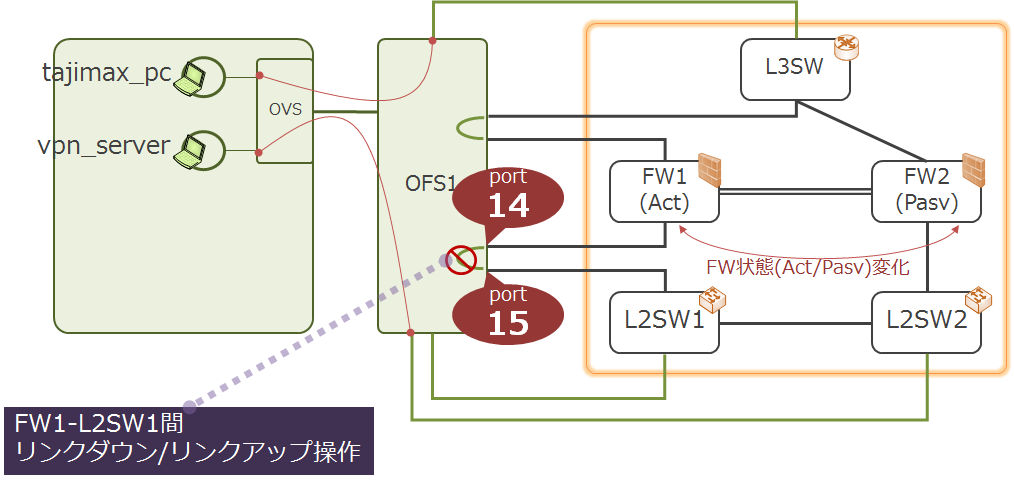
\includegraphics[scale=0.6]{img/poc-env-linkdown.png}
 \caption{PoC環境: NetTesterによるリンクダウン操作}
 \label{fig:poc-env-linkdown}
\end{figure}

  \subsection{継続的通信テストの実装}

テスト対象ネットワークの状態変化を調査する際によく使用されるのは、
Ping(ICMP)を一定間隔で送受信しておき、通信断等の影響がどの程度発生したか
を測定することである。L4(TCP)レベルの情報を同期してフェイルオーバー/フェ
イルバックするFWがある。そのため、L3(ICMP)レベルで通信維持を確認するだけ
でなく、ネットワーク状態変化によるL4レベルでの通信影響も測定する
(\ref{sec:dynamic-test-target}節)。L4レベル影響測定のために、TCPセッショ
ンを張ったままPing同等の動作をおこなうためのツールを自製
\footnote{\url{https://github.com/net-tester/examples/blob/feature/ood_demo/features/support/echo_server.pl}}
して使用している。

リンク障害発生時のトラフィック影響としては、単純に ICMP/TCP ping ログに
おいてパケットが受信できなかった部分の時間差分を計算する
\footnote{\url{https://github.com/net-tester/examples/blob/feature/ood_demo/features/step_definitions/util.rb},
\code{check\_connection}参照。}ことでおこなっている。

  \subsection{動的なふるまいのテストとして実現できたこと}
  \label{sec:dynamic-test-result}

動的なふるまいのテストとして、ICMP/TCP でトラフィックを継続的に流しなが
らFWのフェイルオーバー・フェイルバックをくりかえすテストを実装することが
できた。PoC環境において、FWフェイルオーバー・フェイルバックの動作で問題
(テスト対象NWの不備)は特に発生しなかった。テスターおよびテストシナリオ実
装上のポイントについては\ref{sec:testscenario-impl-point}節にまとめる。

テストシナリオ実装を通して、ネットワーク通信仕様の変更が発生した際の対応
プロセスについても検討している。今回は、\tj からの SSLVPN NAT IP の変更
を題材としている。IP変更要求に対して、以下の手順でテストファーストに対応
を進めるためのデモンストレーション~\cite{nettester-demo-movie}を作成した。
\begin{itemize}
 \item 変更要求にしたがって、対応するテストシナリオを修正する。
 \item テストを実行する。(失敗するテストを書く)
 \item テスト対象ネットワークの設定を変更要求に基づいて変更する。(テスト
       対象の実装)
 \item テストを実行する。(テストが通ることを確認する)
 \item 変更対象のサービス(要求仕様/ふるまい)に影響を与えていないことを確
       認するため、その他のテストシナリオをすべて再実行する。(回帰テスト
       の実行)
\end{itemize}
これにより、要求変化へテストファーストな方法で対応することができた。また、
回帰テストによって、仕様変更後のサービス影響を確認(予期しない影響が発生
していないこと)できた。

 \section{テストシナリオ実装における検討ポイント}
 \label{sec:testscenario-impl-point}

  \subsection{Teardown処理}
  \label{sec:teardown}
CI/CDといったプロセスを実現する上で、複数・任意のテストシナリオをまとめ
て実行することが求められる(回帰テスト含む)。

テストシナリオはいずれも、テスト対象が所定の初期状態にあるところから実行
を開始しなければ狙った「ふるまい」を調査することができない。ソフトウェア
の自動テストでは、テスト対象となるアプリケーション(プロセス)やインスタン
スは初期状態で起動しなおすことが容易である。したがって、常にアプリケーショ
ンやインスタンスを起動しなおして初期状態からのテストをおこなうのが一般的
である。

しかし、ネットワーク(特に物理ネットワーク)を対象としている場合はテスト対
象が物理的に存在している。よって、そのままでは、あるテストシナリオ実行後
のネットワーク状態が、次のテストシナリオを開始する際の初期状態となってし
まう。個々のテストシナリオを実行するたびにネットワーク(機器)の初期化・再
構築することは、不可能ではないが以下の理由により難しい。
\begin{itemize}
 \item 機器によっては、コンフィグ消去・再起動に数分から十数分かかるもの
       がある。
 \item 再起動によるteardown処理をおこなう場合、ネットワーク機器の起動順
       序によりネットワーク全体の状態が変化し得る。
 \item コンフィグリセット操作に失敗すると再起動後にリモートアクセスでき
       ず、復旧作業(現地作業)が必要になるリスクがある。
\end{itemize}
特に本PoCでは、静的なふるまいのテストとして数十の通信要件をテストするた
めのシナリオを連続実行したいという要求があるため、単一テストシナリオ実行
の時間的なオーバーヘッドが大きいことが問題となる。

よって、テストに応じて何らかの形でネットワークの状態を初期状態に戻すため
の処理(teardown処理)を実装する必要がある。本PoCではL2--L4の状態に着目し
て、以下のteardown操作を実装している。

    \paragraph{テスト対象ネットワークの状態操作}
テスト対象ネットワークにある各機器のL2--L4状態をクリアする(CLIによる各種
\code{clear}コマンドの実行)。
\begin{itemize}
 \item MACアドレステーブル/ARPキャッシュのクリア
 \item FWの NAT Table のクリア
 \item FWの active/standby 状態のクリア
       \begin{itemize}
        \item 今回、動的なふるまいのテストにあたって、FWは障害が発生した
              リンク復旧時に active/passive を自動変更するよう設計した
              (\ref{sec:physical_nw_design}節)。そのため、特にテストシナ
              リオ内では操作していない。
       \end{itemize}
\end{itemize}

    \paragraph{Netns の /etc 配下のSetup/Teardown}
    % 自作echoサーバーで通信開始時に10秒のラグが起きる問題 – NetTester
    % https://3.basecamp.com/3088280/buckets/867009/todos/274457003

NetTesterでは、Network namespace でテスト用ノードを生成する。このときバッ
クエンドでは iproute2(\code{ip}コマンド)を使用している。iproute2 によっ
て生成されたノード(netns)では、\verb|/etc/netns/<netns>/| が etc ディレ
クトリとしてマウントされる~\cite{iproute2-doc}。よって、テスト用ノード内
部での名前解決などでは、実体としては \verb|/etc/netns/<netns>/hosts|,
\verb|resolv.conf| を参照する。これらの設定ファイル等が正しく設定されて
いないと、名前解決がタイムアウトするなどの問題が発生する。

    \paragraph{物理OFSのflow tableのクリア}
物理OpenFlowスイッチには、テストのたびにフローエントリが登録される。その
ため、テスト実行のたびにフローエントリのクリア処理が必要となる。

本PoCでは、テスト用ノードのMACはテスト実行時にランダムに設定するよう実装
したため、テスト実行をくりかえすと多数の不要なフローエントリが物理スイッ
チ上に残る。テスト用ノードのMACアドレスを固定にするとフローテーブルの消
費は抑えられる。しかし、異なる用途で同一のMACアドレスを使いまわすなどの
ケースで、予期しない動作不具合が発生する恐れがある\footnote{NetTesterの
テーブル設計では、テスト用ノードのMACアドレスをキーとして、フロー優先度
(priority)による制御をおこなう(\ref{sec:flow-priority-design}節)。同一
MACアドレスを異なる用途で使いまわす場合、他の用途として設定したフローエ
ントリとマッチしてしまい、狙ったパッチ動作が実現できない恐れがある。}点
に注意すること。

    \paragraph{テスト用ノードのパラメタ設定の考えかた}
    % テスト用ノード(host)のMAC addr を固定にするかどうか方針を決める。 – NetTester
    % https://3.basecamp.com/3088280/buckets/867009/todos/218612153

テスト用ノードのMACアドレス設定による不具合が見付かった際
(\ref{sec:find-nw-device-bug}節)、一時的にテスト用ノードのMACアドレス設
定をテストシナリオ上で固定にすることで回避した。しかし、実際にはteardown
処理を実装し、テスト用ノードのMACアドレスはシナリオ実行時にランダムに設
定されるようにした。これは次のような考えかたによる。
\begin{itemize}
 \item 通常、テスト対象に接続する機器のMACアドレスについて、テスト作業者
       が意識していることはほとんどない。テストシナリオを記述する際にも
       同様に、意識しなくてよいものを意識させなければいけない実装は避け、
       テストシナリオの本質的な部分の実装に注力できるようにすべきである。
       \begin{itemize}
        \item もちろんテストシナリオとして常に指定したMACアドレスを使う
              ことも可能である。テスト対象ネットワーク内の機器について、
              ユニットテストで詳細な動作を調査するような場合にはこうした
              機能が必要になる。
        \item 本PoCでは「ふるまい」つまり要求仕様ベースでのテストを主眼
              においている。よって、そのレベルで本題でないパラメタ設定は
              テストシナリオ実装者に極力意識させないようにする。
       \end{itemize}
 \item 物理的なテスト対象では、テスト対象インスタンスの状態を低コストで
       クリアすることが難しく、teardown処理はテスト自動化において重要な
       処理となる。一時的にMACアドレス等の設定で回避してしまうのではなく、
       PoCを実行するうえで実用性があるかどうかを見極める必要がある。
\end{itemize}

  \subsection{NetTesterおよびテストシナリオの並列実行と排他制御}
  \label{sec:testscenario-excl-ctrl}

物理ネットワークをテストする場合、テスト対象(物理ネットワーク)はひとつし
かない。テストの数が多くなる場合、複数のテストを同時に実行することが考え
られるが、現状NetTesterを使ったテスト自動化では、並行実行は原則できない。
以下にその理由を列挙する。

\begin{description}
 \item[状態操作の競合] テストシナリオごとに、想定しているテスト対象ネッ
            トワークの状態がある。それらを変化させるテストシナリオは同時
            に実行できない。
            \begin{itemize}
             \item シナリオA実行中にシナリオBがteardown処理を実行して、
                   テスト対象ネットワークの状態クリアをしてしまったとす
                   る。すると、シナリオAで想定していた状態を変化させてし
                   まう\footnote{Teardown処理として\code{clear}コマンド
                   を使用しているが、特定シナリオで使うエントリだけを消
                   去するのではなく、NW機器全体の情報をまとめて消去して
                   しまうため。そのシナリオに依存するエントリだけをねらっ
                   て消去できるのであればこの制約は外れるが、テスト対象
                   ネットワーク内の機器それぞれについて対応可能かどうか
                   という点が問題となるだろう。あるいは、teardown処理を
                   他のテストシナリオ実行がおわるまで待機し、まとめて実
                   行できればよいが、現状はそうした実装をおこなっていな
                   い。}。
             \item 動的なふるまいのテスト同様、ネットワーク全体の状態に
                   影響をあたえるようなテストシナリオは同時に実行できな
                   い。
            \end{itemize}
 \item[ネットワークリソースの競合] テスト対象ネットワークで一意でなけれ
            ばならないリソースの操作については同時に実行できない。
            \begin{itemize}
             \item シナリオA,Bが同じIP/MACを持つテスト用ノードを同時に生
                   成してしまったとする。この場合、テスト対象ネットワー
                   ク内でIP/MACの重複が発生してしまう。
             \item 物理リンクの操作など、ひとつしか存在しないリソースの
                   制御が必要なテストシナリオは同時に実行できない。
            \end{itemize}
\end{description}

本PoCでは\figref{fig:poc-env-physical-detail}のようにふたつのtester set
を使用しているが、これはあくまでもデバッグ用途のためである。Tester set
を複数用意すると、
\begin{itemize}
 \item 静的なふるまいのテスト(NWが定常状態にある)を
 \item 同じIP/MACのテスト用ノードを使用しない
 \item teardown 処理をテストシナリオ単位で実行しない
\end{itemize}
ようなケースに限って同時にテストシナリオが実行可能となる。

上記の制約については、NetTesterで実行されるタスクを排他制御するしくみを
導入することで対応できるものがあるが、現状はそうした対応については本PoC
の範囲外としている。本PoCでは、ひとつのテスト対象ネットワークに対して
tester setがあり、同時にひとつのテストシナリオを実行することが前提となっ
ている。

  \subsection{テストダブルの考えかた}
  % ニセ○○サーバとステップ実装 – NetTester
  % https://3.basecamp.com/3088280/buckets/867009/documents/216490375
一般的に、ソフトウェアテストにおいて、テスト対象が依存しているコンポーネ
ントを置き換える代用品のことをテストダブル~\cite{test-double}という。

本PoCのように、end-to-end のネットワークテストをおこなう場合、テストトラ
フィック生成のためにクライアント/サーバを用意する必要がある。テスト対象
ネットワーク内に既存のサーバがあるケースもあれば、本PoCのように実際には
サーバがなく、代替となるサーバをテストシナリオで準備しなければならないケー
スもある。

テストダブルとしてのサーバを導入する場合、導入することによって他のテスト
コード書き換えが発生する\footnote{実際のサーバがある場合のテストコードと
代替サーバを使う場合のテストコードが大きく異なる}のは好ましくない。

例として、インターネット検索(google)の可否をテストする場合をとりあげる。
テスト対象ネットワークが直接インターネットアクセス可能で直接googleのウェ
ブサイトを見ることができる場合、\lstref{lst:real-service-test}のようなス
テップにできる。テスト対象ネットワークが直接インターネットアクセスできな
い場合は、テストダブルを建てて\lstref{lst:testdouble-test}としたとする。

\begin{lstlisting}[caption=実際のサービスを利用する場合,label=lst:real-service-test]
When(/^ブラウザで Google のページを開く$/) do
  cd('.') do
    @browser_pc.exec 'curl -L https://google.com/ > log/google.log'
  end
end

Then(/^Web サイトへのアクセスに成功$/) do
   step %(the file "log/google.log" should contain "<title>Google</title>")
end
\end{lstlisting}

\begin{lstlisting}[caption=テストダブルを利用する場合,label=lst:testdouble-test]
When(/^ブラウザで Google のページを開く$/) do
  cd('.') do
    @browser_pc.exec "nc 192.0.2.100 80 > log/nc_web.log"
  end
end

Then(/^Web サイトへのアクセスに成功$/) do
  step %(the file "log/nc_web.log" should contain "OK")
end
\end{lstlisting}

\lstref{lst:testdouble-test}では、テストダブルを使用することでサーバにつ
いてのコードを変更しているが、それだけでなくクライアント側の処理に関する
コードにも影響をあたえてしまっている。「ふるまい」として「googleに接続し
て検索したい」という目的をふまえると、\lstref{lst:real-service-test}では
直接的に「検索サービスに接続」していることがわかる。ところが、テストダブ
ルを導入した\lstref{lst:testdouble-test}では、本来テストしたい「ふるまい」
を間接的にしか表現できていない。

しかし実際には、テストダブルで代替したい元のサービスを完全に実現すること
は不可能である(簡単にオリジナルのサーバを準備できるのであればテストダブ
ルを準備する必要がない)。本PoCでは、例えば
\tabref{tab:poc-requires-yo-int} No.1 では git を使用する要件がある。実
際に \verb|git clone|コマンドでリポジトリ操作可能かどうか(L7)というレベ
ルでテストする、TCP(L4)レベルの接続性だけをテストするなど、複数の方法が
考えられる。テストの目的(テストしたいことは何か)に対して、どこまでを保証
するのかという線引きをテスト自動化システムのポリシとして設定しておく必要
がある。

  \subsection{コマンドのバックグラウンド実行}
  \label{sec:background-exec-method}
  % コマンドをバックグラウンド実行 – NetTester
  % https://3.basecamp.com/3088280/buckets/867009/documents/216399643
  % step内でのバックグラウンドコマンド実行 – NetTester
  % https://3.basecamp.com/3088280/buckets/867009/todos/202691188

例えば次のような場合に、並列でコマンドを実行する・クライアント操作が終了
したらサーバを終了する、などの処理が必要になる。こうしたテストの実装では、
単発の同期コマンド実行(\verb|exec|)ではなく、非同期で実行し、joinさせる
ような手段が求められる。
\begin{itemize}
 \item テスト用ノードでのサーバプロセス実行 (テストダブルの生成)
 \item 動的なふるまいのテストにおける複数トラフィックの同時生成
\end{itemize}

NetTesterを使ったテストステップの実装では、バックグラウンド実行の方法と
してふたつの方法がある\footnote{\code{Netns\#exec}でバックグラウンド実行
することはできない。これは\code{Netns\#exec}が内部的に利用している
\code{Open3.popen3}の仕様によるものである。}。
\begin{description}
 \item[スレッドを使う] \verb|#exec|自体を別スレッドで動かす。
\begin{lstlisting}
Thread.start { @server.exec "bash -c 'echo OK | nc -l 80'" }
\end{lstlisting}
 \item[直接ipコマンドを使う] \verb|Netns#exec|と同様のことを\verb|ip|コ
            マンドを使って直接バックグラウンド実行する
\begin{lstlisting}
run "sudo ip netns exec #{@server.name} bash -c 'echo OK | nc -l 80 &'"
\end{lstlisting}
\end{description}

本PoCではスレッドを使う方法を採用し、\verb|AsyncExecutor|クラス
\footnote{\url{https://github.com/net-tester/examples/blob/develop/features/support/async_executor.rb}}
を用意してテスト用ノード上でのバックグラウンドコマンド実行をおこなってい
る。

  \subsection{テスト用ノードのパラメタ管理}
  \label{sec:test-parameter-management}
  % factory_girl で仮想ホストを作る – NetTester
  % https://3.basecamp.com/3088280/buckets/867009/documents/210831650

\lstref{lst:nettester_basic_example}で、NetTester の基本的な仕様方法をサ
ンプルコードで示した。NetTester でテスト用ノードを生成する
(\verb|NetTester#new|)場合、テスト用ノードが持つIPアドレス等各種パラメタ
を設定する必要がある。これらのパラメタは複数のテストシナリオにまたがって
使用されたり、テスト結果によっては変更されることがある。そのため、
\lstref{lst:nettester_basic_example}に示すような直接的なパラメタ記述では
管理が煩雑になってしまう。

そこで、テストデータの管理に Factory Girl~\cite{factory-girl}を使用する。
各テストシナリオで使用するテストデータを
\verb|features/factories.rb|\footnote{\url{https://github.com/net-tester/examples/blob/develop/features/factories.rb}}
で管理する。\verb|factories.rb|では次の情報を記述する。
\begin{description}
 \item[仮想ノード共通属性の定義] ネットワークアドレスやゲートウェイのよ
            うに、各テスト用ノードが共有する属性を記述する。
\begin{lstlisting}
FactoryGirl.define do
  trait :internal_network_host do
    netmask '255.255.255.0'
    gateway '10.10.10.254'
    mac_address Faker::Internet.mac_address('00')
  end

 ...
end
\end{lstlisting}
 \item[仮想ノードの定義] すでに定義した \verb|:internal_network_host| 使っ
            て仮想ノードを生成する。
\begin{lstlisting}
FactoryGirl.define do
  ...

  factory :ntp_client, class: Netns do
    internal_network_host

    name 'ntp_client'
    ip_address '10.10.10.3'
    virtual_port_number 2
    physical_port_number 2
  end
end
\end{lstlisting}
\end{description}

Factory Girl で定義されたテストデータを使用してテスト用ノードを生成する
と次のようになる。このように、テスト用ノードの共通パラメタを分離し、本質
的でないパラメタの隠蔽できる。
\begin{lstlisting}
Given(/^NTP クライアントとなる開発者 PC$/) do
  @ntp_client = Netns.new(attributes_for(:ntp_client))
end
\end{lstlisting}

  \subsection{テストシナリオのサイズ}

% シナリオサイズの目安、シナリオ分割の目安 (step3 test つくっているときに
% 分割するって話になった理由は?)
% Answer to “今日なにした?” – NetTester
% https://3.basecamp.com/3088280/buckets/867009/question_answers/267488304
% 集中作業日1 – NetTester
% https://3.basecamp.com/3088280/buckets/867009/schedule_entries/260224157

動的なふるまいのテスト(リンク障害試験)について、手作業で実施する場合には、
1回のイベント(リンクダウンまたはリンクアップの発生)に対して複数の操作を
おこなう。例えば、あらかじめ複数のテストトラフィックを生成しておき(今回
のPoCシナリオでは複数パスの ICMP/TCP pingの実行)、1回のイベントに対して
それらのトラフィックがどう変化したのかを確認する。

これをそのままテストシナリオとして記述すると、ひとつのシナリオのステップ
数が増大し、テストシナリオ全体の見通しが悪くなってしまう。そこで本PoCで
は、テストが繰り返し実行可能であることを利用して、イベント・トラフィック
ごとにテストのシナリオを分割し、ひとつひとつのテストシナリオが単純かつ理
解しやすいものになるようにした。

手作業でテストシナリオを実行する場合には、くりかえし実行(作業)する時間的
コストが大きいためイベントの発生回数自体をおさえる。しかし、テストシナリ
オを自動化した場合は、繰り返し実行することのコストは低い。そのため手作業
で実行する際の一般的なやりかたに準拠させる必要はなく、個々のテストシナリ
オのメンテナンス性を重視して考えることができる。

  \subsection{Sleep tuning}
  \label{sec:sleep-tuning}
% step3 テストにおけるsleep調整など、課題、対応について。

テストシナリオ(テストステップ)の実装にあたっては、処理のタイミングを同期
させるために sleep によるタイミング調整が必要になる。
\begin{itemize}
 \item 処理の待機
       \begin{itemize}
        \item 物理OFSとOFCとの接続・再接続の待機
        \item テスト対象機器に対するコマンドの発行、処理実行の待機
        \item コマンド実行後のログファイル生成等の待機
        \item スレッドによるコマンドの同時実行
              (\ref{sec:background-exec-method}節)を使用する場合は、スレッ
              ドのスケジューリングのためにコマンド実行までにタイムラグが
              あるため sleep を設定する。
       \end{itemize}
 \item テストシナリオ上必要な操作タイミング設定
       \begin{itemize}
        \item 動的なふるまいのテストの場合は、イベント発生前・発生後の定
              常状態遷移待機(テスト対象ネットワークのトポロジの収束など)
              のように、テスト対象の状態変化にかかる時間にあわせたテスト
              オペレーション実行タイミング調整が必要になる。
       \end{itemize}
\end{itemize}

テストシナリオ上必要なタイミング設定についてはテストステップとして明示的
にテストシナリオ中に待機時間を明示する。
\begin{lstlisting}
When(/^(\d+) 秒待つ$/) do |seconds|
  sleep seconds.to_i
end
\end{lstlisting}

処理の待機について、テストシナリオの実行と本質的に無関係のものであればテ
ストシナリオ上は明示させる必要がない。テストステップ中での sleep 実装は
意図や必要性がわかりにくくなりがちであるため乱用には注意が必要である。ま
た、デバッグのために一時的にsleepを設定することがある\footnote{一時的に
テストシナリオ実行を遅延させて別途テスト対象ネットワーク上での調査や作業
をおこなう}ようなケースでは不要なsleepチューニングが残らないようにする必
要がある。

  \subsection{標準出力(stdout)の操作}
  % 今日なにした? – NetTester
  % https://3.basecamp.com/3088280/buckets/867009/questions/181826801/answers/2016-10-21#__recording_267488304
テストステップ実装では、テスト用ノードのコマンド実行結果(stdout)を取得し
たいケースがある。このとき、\verb|$stdout|の操作をおこなってしまうと、
teardown処理等で実行するexpect系ツールへ影響を与えてしまうことがある。

今回、テスト対象ネットワークの操作にはexpectacle(\ref{sec:expectacle}節)
を使用しているが、内部的には \code{spawn} されたコマンド
(\code{telnet},\code{ssh})の標準出力を\code{pty}/\code{expect}で操作して
いる。テストシナリオ(テストステップ)側で \verb|$stdout| などを操作してし
まうと、こうしたプロセスに影響が及んでしまう点に注意すること。

 \section{テストシナリオのデバッグ}

  \subsection{テスト失敗の要因}
テストシナリオの実装・実行をした際、テストが失敗したときには原因として以
下の要因が考えられる(\ref{sec:statictest-founded-issues}節)。また、これ
らの原因が複合して発生することがある。
\begin{description}
 \item[テストシナリオ実装とテスト対象ネットワーク実装の認識違い] テスト
            実装者とテスト対象ネットワーク構築者との認識違い。
 \item[テスト対象ネットワークの設計や設定の不備] テストの目的通り、テス
            ト対象が仕様を実現できていないこと、予期しない動作を発見でき
            ている状態。
 \item[テストシナリオの実装上の不備] テストシナリオ・テストステップ実装
            上の不備。テストに仕様するツールやコマンドの実行時エラーやシ
            ナリオ全体としてみたときのテストオペレーション実行タイミング
            のずれ・ログ取得不備など。
 \item[テスター(NetTester)の動作不具合] NetTester実装においてはテスター
            自体の不具合やバグなどが発生する。
\end{description}

  \subsection{テスト失敗の原因切り分け}
% 原因切り分けのメモを書く – NetTester
% https://3.basecamp.com/3088280/buckets/867009/todos/214926110
% 原因切り分けメモ (muraki) – NetTester
% https://3.basecamp.com/3088280/buckets/867009/documents/217782147

テストが失敗した場合は、まずは問題がテスター側にあるのかテスト対象ネット
ワーク側にあるのかを切り分ける必要がある。以下に問題切り分け・デバッグ時
の確認ポイントを示す。

    \paragraph{テスト対象ネットワーク側での操作}

\begin{itemize}
 \item テスト用ノードが生成したトラフィックがテスト対象ネットワークに届
       いているかどうかを、ARP/MACアドレステーブルで確認する。テスター側
       のVLAN設定とテスト対象ネットワーク機器側のポートVLAN設定とのミス
       マッチに注意すること。
 \item テスト用ノード接続ポートのパケットカウンタ(エラーカウンタ)を確認
       する。
 \item ステートフルファイアウォールでは、policy別のセッション状況を確認
       する。\footnote{Juniper SSG の場合は\code{get log traffic}コマン
       ドで確認できる。}
 \item テスト対象ネットワーク機器でテスト用ノードが生成したトラフィック
       が送受信できていない場合はパケットキャプチャしてヘッダ等の情報を
       確認する。(NetTesterの場合、L2(MAC, VLAN Tag)操作する点に注意。)
\end{itemize}

    \paragraph{テスター側OVSでの操作}

\begin{itemize}
 \item OVSのポート通信量を確認する。テスト対象ネットワーク機器側とあわせ
       て確認することで、L1/L2レベルでの接続状態を確認する。
\begin{lstlisting}
ovs-ofctl dump-ports <bridge> <port-number>
\end{lstlisting}
 \item フローテーブル、フローエントリに対するパケットカウンタの確認: フ
       ローテーブル設計・実装のデバッグをおこなう\footnote{2016年12月時
       点では、NetTesterはOFSのteardown処理を実装していない。過去のテス
       トの際にフローテーブルに残ったエントリによる影響なども考慮に入れ
       る必要がある(\ref{sec:teardown}節)。}。
\begin{lstlisting}
ovs-ofctl dump-ports <bridge>
\end{lstlisting}
 \item OFS-OFC間通信(セキュアチャネル)状態および送受信されるOpenFlow
       Messageの確認
\begin{lstlisting}
ovs-vsctl snoop <bridge>
\end{lstlisting}
\end{itemize}

    \paragraph{テスター(NetTester)サーバでの操作}

\begin{itemize}
 \item PSW-SSW間リンクでのパケットキャプチャ実行。NetTesterサーバのOFSス
       イッチ接続ポート\footnote{\figref{fig:nettester-deploy-vm}のens5
       相当のインタフェース}で、全テスト用ノードのトラフィックをキャプチャ
       できる。
 \item テスト用ノードの ARP テーブルの確認
 \item NetTester OFC(trema)でのデバッグ: \ref{sec:debugging-trema}節参照。
 \item OS上での不要な network namespace や veth インタフェース等の確認
\end{itemize}

    \paragraph{テストシナリオでの操作}

\begin{itemize}
 \item Pry~\cite{pry}によるデバッグ実行。テストシナリオ(ステップ)中にpry
       を挿入することでインタラクティブシェルに移行する。シェル上でテス
       トシナリオ上の変数やテスト対象ネットワークの状態などを確認する。
 \item 各テストオペレーションでの操作ログ取得
 \item Sleep tuning, テストシナリオの連続(繰り返し実行)や実行間隔の調整。
       キャッシュ依存の動作やタイマベースの状態変化イベントなどでは、テ
       ストの実行タイミングあるいは実行順序によってテスト実行結果が変化
       することがある。
\end{itemize}

  \subsection{テスト対象ネットワークを含めた原因調査}

テストシナリオが失敗(Fail)した原因を調査する際、テスター側の動作状況・ロ
グだけでなく、テスト対象ネットワーク内の各機器に対するオペレーションや状
態変化ログもあわせて一元管理できることが望ましい。そのために、一般的なネッ
トワークのテスト実行や検証作業と同様、テスト対象ネットワーク機器のログ
(Syslog)収集、時刻同期(NTP)などを実施しておくことが必要である。この他、
テスト環境としては以下のような点が検討事項となる。
\begin{itemize}
 \item テスト自動化としては、物理構成の操作を極力避けたいという狙いがあ
       る。テスト環境構成の際にはあらかじめ、パケットキャプチャ用のリソー
       スや予備配線などを想定した設計をしておくことが望ましい。
 \item 問題切り分け用の対照設定・対照機器を準備する。今回テストシナリオ
       実装にあたっては、FWのパケットフィルタを設定していない(permit
       any)FWを1台用意した。この機器を使用して、テスト用ノード
       (server/client)が直接通信してテストが実行可能かどうか切りわけ作業
       を実施した。テストシナリオを一度に作成してテスト実行可否を見極め
       るのが難しい場合は、テストシナリオ自体の段階的な動作確認や切り分
       けの工夫が求められる。
\end{itemize}

 \section{テストシナリオのリファクタリング}
 % リファクタリング内容のサマリを作る – NetTester
 % https://3.basecamp.com/3088280/buckets/867009/todos/421050078

実際に作成したテストシナリオについてどのような課題があったか、それをどの
ように改善(リファクタリング)したのかについて説明する。

  \subsection{ファイル名}

実装当初、テストシナリオのファイル名やディレクトリ(階層)にどのような情報
を持たせるかを決定しきれていなかった。そのため、ファイルがどのテストシナ
リオを指しているのかが不明瞭になってしまった。

    \paragraph{テストシナリオのファイル名}
通信試験(静的なふるまいのテスト)で実際にファイル名に使用されている要素は
次の通りである。
\begin{itemize}
 \item 機能 (サービス)
 \item 視点 (Narrativeにおける ``As a ...'' に相当)
 \item 送信元セグメント
 \item 送信元ホスト
 \item 送信先セグメント
 \item 送信先ホスト
\end{itemize}
テストシナリオ(feature)のファイル名は当初、\code{機能名.feature}という形
で作成しはじめた。しかし、通信試験では機能名は同一だが実行するセグメント
が異なるテストが存在するため、\code{from\_to\_機能.feature}というファイ
ル名で区別するようになった。このときにファイル名のルールが明確でなく、使
われる単語や順序に統一性をもたせることができていなかった。

そこで、テストシナリオのリファクタリングをすすめる中で、\code{feature/視
点/送信元ホスト\_to\_送信先ホスト/機能(サービス).feature} という形式に統一
した。

    \paragraph{テストステップのファイル名}
テストステップ(具体的なテスト操作)については、ある程度の量テストシナリオ
を実装してテストの粒度・サイズ・パターンなどを把握することが難しかった。
そのため、どのような単位でstepに分けるべきか判断できず、実施内容と成功判
断が混在(しかも個別に存在)するようなstepが乱立した。

ホストの起動に関しては、初期は機能ごとのstepに書き始めたが、同じものが出
てくるため早い段階で \verb|virtual_host.rb| でまとめて書くようになった。
それでも、\verb|internal_pc| と \verb|git_client| など、役割が重複するも
のが乱立していた機能があった。

機能に関しては \verb|機能(サービス)_steps.rb| だけの状態から始まり、徐々
にテスト結果判定を \verb|(確認内容)_success_steps.rb| に切り出す形になっ
た。しかし、用語や記述の統一が曖昧だったため、中身は feature ごとの制御
や確認が複数ある状態だった。最終的に、用語を統一するリファクタリングで、
実施内容・確認内容の重複が排除していった。

  \subsection{視点の統一}
テストシナリオが誰の視点なのかわからない始まり方をし、何をしたいのかが曖
昧なテストシナリオがあった。視点が曖昧になってしまったテストシナリオにつ
いては次のように視点を明確化させるようにした。
\begin{itemize}
 \item テスト対象ネットワークを使うのは誰か、登場人物として「利用者」と
       「管理者」に分けて考えることにした。
 \item まずは利用者目線のものから、間で何が行われているかを気にせず、や
       りたいことは何かを確認する形でテストシナリオを作成する。
 \item 管理者ではやりたいことが利用者と異なりサービスが提供できることが
       やりたいことだと定義してテストシナリオを作成する。
\end{itemize}
ネットワークを利用するのは利用者(エンドユーザ、すなわち \yo 社員)だけで
はなく、ネットワーク管理者なども含まれる。誰の視点でテストが必要なのか、
登場人物とその目的(つまりNarrativeで記述するテストの観点)を整理すること
でテストシナリオの必要性を明示するようにした。

\subsection{命名規則}
登場人物については整理したが、テストシナリオの実装(表記)について明確なルー
ルは設定できていなかった。複数人での並行開発により、同じことをしたいstep
でも記述に揺れ、重複するファイル名やfeatureが発生した。また、stepに同義
語が多く登場するようになってしまった。問題となった同義語には次のようなも
のである。
\begin{itemize}
 \item 企業名の表記
 \item ホスト名なのか機能名(サービス名)なのか
 \item プロトコル名なのか機能名(サービス名)なのか
 \item セグメントなのかホストなのか
       \begin{itemize}
        \item 記述のしかた自体も不明確なものも。
        \item 例: 内部, ヨーヨーダイン社内
        \item 例: クライアント, Xするクライアント, クライアントPC, ユー
              ザPC
        \item 例: DMZのサーバ, DMZ内のサーバ, DMZ内部のサーバ
       \end{itemize}
\end{itemize}
こうした同義語については、リファクタリングする際に調査とルールを作り、用
語・用法の統一をおこなった。
\begin{itemize}
 \item 企業名
 \item セグメント日本語名
 \item ホスト日本語名
 \item ホストインスタンス名
 \item 機能(サービス)名
       \begin{itemize}
        \item HTTPSやhttpsなどの文字統一性がなかった点もルールを決めて統一
       \end{itemize}
 \item サービスとホストの区分け
       \begin{itemize}
        \item クライアントマシン: \verb|hoge_pc|
        \item サーバマシン: \verb|hoge_host|
        \item サーバサービス(AsyncExecutor): \verb|hoge_service|
       \end{itemize}
\end{itemize}

  \subsection{機能・サービス名やテストシナリオの言葉づかい}

テストシナリオを先行実装した際に、通信要件上、何のサービスなのか具体的で
ないキーワードが存在した。こうした用語があると、テストシナリオで何をした
いものなのかが一読してわからなくなってしまうため、実際に使う機能(サービ
ス)名で明示するようにした。例えば、アプリケーション名としてAP1, AP2など
の用語を使用していた。AP1(資産管理)はgit、AP2(内部テストサーバ)はjenkins
などのように実際の機能として明示している。

また、PoCの位置付けとしてSIerによるシステム構築というPoCシナリオを想定し
ていたことから、全体的に固い単語や言い回しが多かった。「疎通確認」「経由」
などSIやシステム管理者・ネトワークエンジニアでなければなじみの薄い用語は
極力使用せず、平易な言葉に置き換えた。

テストシナリオ(feature)自体にも、文脈を明確にするため全節に補語を記述し、
「\yo 」という言葉が何度も登場していた。そのためシナリオ全体が冗長で読み
にくいものになってしまった\footnote{「\yo から \yo 内部のテスト環境サー
バへsshでログイン」などの文言が多発していた。}。そこで、
\tabref{tab:basic_scenario}の形で上から文脈を固定していくようにした。こ
うすることで、テストシナリオの文脈を明確にしつつ冗長な表現を避け、シンプ
ルで平易なシナリオになった。
\begin{table}[h]
 \centering
 \caption{通信テストの基本シナリオ}
 \label{tab:basic_scenario}
 \begin{tabular}[t]{l|l|l}
  \hline
  Step Keyword & Step & Step detail \\
  \hline
  \hline
  Given & Source & Sourceのホストを作る \\
  And   & Destination & Destinationのホストを作る \\
  When  & Sourceにログイン & \verb|@src_host|にSourceをいれる \\
  And   & テスト実行 & Destinationのサービスを起動、\verb|@src_host|からアクセス \\
  Then & 確認 & テスト実行結果を確認し、成否を判定する \\
  \hline
 \end{tabular}
\end{table}


  \subsection{テストクライアント実行手段・成否判断}
  \label{sec:test-client-exec}

    \paragraph{並行実行の方式}

複数コマンドの並行実行(\ref{sec:background-exec-method}節)は実装方式を徐々
に変更している。最初はバックグラウンド実行(\verb|command &|)で実装し、中
盤からAsyncExecutorに変更している。ただし、リファクタリングするまでいく
つかバックグラウンド実行の実装が残ってしまっていたため、AsyncExecutorに
統一した。

    \paragraph{テストに使用するツール}
% system.exec(hoge&)を探す – NetTester
% https://3.basecamp.com/3088280/buckets/867009/todos/384120258

初期はnetcat (\verb|nc|)を使用してL4レベルの通信テストを実装していた。し
かし、実際に使用するツールやサービスを使えるのであれば、可能な限り実際に
利用者・管理者が実施するオペレーション近づけるようにした。そこで、
dnsmasqや、openssl/sshdをstep実装のなかで使うようになった。ただし、利用
するツールの特性に応じて以下のような変更を加えている。
\begin{itemize}
 \item 対話型コマンドを排除するため、opensslを使用していた実装はWEBrick
       へ置き換えた。
 \item Telnetなどの単純なTCP通信試験にはnetcatをサーバ使用している。しか
       し、telnetクライアントとサーバ(\verb|nc|)間でメッセージを送受信す
       る順序によって、おなじテストでも成功・失敗が安定しない事象が発生
       した(\ref{sec:telnet-probrem}節)。そのため、telnetクライアントは
       \code{telnet}コマンドではなくNet::Telnetを使用している。
\end{itemize}
% TBA: 別途バッドノウハウ系の話を追記。
% telnetが1/10くらいしか成功しない – NetTester https://3.basecamp.com/3088280/buckets/867009/todos/411777005

\paragraph{NetTester固有のテストシナリオ実装}
NetTesterを利用してテストシナリオを実装する際には、ホストの仮想ポート番
号を考慮しなければならない。テストシナリオ作成上重要なのは、テストノード
をテスト対象ネットワークのどこに接続させるかである。テストノードが
OVS(ssw)のどこに接続するか\footnote{\code{virtual\_port},
\ref{sec:nettester-api-basics}節、\ref{sec:test-parameter-management}節
参照。}を意識する必要はないため、OVS側のポート番号は\verb|sequence|で自
動的に採番(連番)する機能を実装している。

  \subsection{Cucumberの活用}
% static/dynamicタグの名前を直す – NetTester
% https://3.basecamp.com/3088280/buckets/867009/todos/442878606

    \paragraph{タグによる実行テストシナリオのフィルタリング}
Cucumberは指定したルール(タグ式)でテストシナリオを実行する機能を持ってい
る。現時点(2017年3月)時点では\tabref{tab:scenario_tags}に示すタグをテス
トシナリオに設定している。いくつかのタグについて、そのタグを設定するまで
の経緯を示す。テストの事項単位や種別ごとにタグを設定することで、特定のテ
ストシナリオだけをフィルタして実行できる。

\begin{table}[h]
 \centering
 \caption{使用しているタグとその用途}
 \label{tab:scenario_tags}
 \begin{tabularx}{\linewidth}{p{10em}|X}
  \hline
  タグ & 用途 \\
  \hline
  \hline
  \verb|@wip| & Work In Progress, 作成途中のテストシナリオに付与して実行スキップさせる。\\ \hline
  \verb|@demo| & デモ用にいくつかのシナリオをまとめて実行するために付与。一時的な利用だったのでその後削除。 \\ \hline
  \verb|@internet| & テスト対象ネットワークにインターネット接続がある前提のテスト・インターネット接続がない前提のテストを区別するために設定。最初は\verb|@nointernet|というタグも設定していた。しかし、\verb|@nointernet|のような否定型タグは意味がわかりにくく\footnote{Cucumberのタグ式では否定の論理演算(NOT)も使用できるため二重否定の式になってしまう。}なってしまう。そのためデフォルトをインターネット接続なしとし、テスト対象ネットワークにインターネット接続がある場合のみ \verb|@internet|タグを指定する形に変更した。 \\ \hline
  \verb|@static_topology|, \verb|@failure_recovery| & \verb|@static_topology|は静的なふるまいのテスト(通信試験)、\verb|@failure_recovery|は動的なふるまいのテスト(障害試験)に付与する。最初はそれぞれ \verb|@static|, \verb|@dynamic|というタグだったが、タグ単体でみたときの意図が不明確なので、より具体的なテスト条件がわかる用語へと置き換えている。\\
  \hline
 \end{tabularx}
\end{table}

\paragraph{テストステップの自動補完}

Cucumber には、テストシナリオに対するステップ実装がない場合、シナリオ(文)を
もとにテストの雛形を生成する機能がある。この機能を利用するためには 英数
字(単語)の前後にブランクが必要になる。リファクタリングの中ではNarrative
含め英数字前後はブランクありで統一し、テストシナリオ作成時のルールとして
設定している。

\section{PoC結果に関する定性的な評価}
% 評価・考察
% - 体制や役割分担/タスクとスキルセットについて
%   https://3.basecamp.com/3088280/buckets/867009/todos/260220903
% - テスト実装のコスト
% - 繰り返し実行できることのメリット
%   - OSの更新などおおきな変更にたいするリスクヘッジ

本PoCでは、BDDという考えかたのもとに、静的・動的なふるまいのテストを実装
した。実際に、これまで手作業でおこなってきたのと同等の end-to-end 通信試
験やリンク障害試験を自動化することができた。また、teardown処理の難しさな
ど、ソフトウェア開発における自動テストでは存在しない(物理ネットワークの
テストに固有な)問題などもあきらかにすることができた。本節ではテスト自動
化システムの運用に付随する検討事項や当初目的に対する今後の課題について解
説する。

  \subsection{ネットワークの構築・運用プロセス}

本プロジェクトの目的としてはネットワークの構築・運用プロセスのCI/CD化
(\ref{sec:network-test-and-process}節)がある。今回、
\ref{sec:dynamic-test-result}節に示したように、テストファーストな運用と
いう観点での操作を実際に試している。この中で、テストシナリオによる回帰テ
ストの実行と影響範囲のチェックはできている。CIの最も基本的なオペレーショ
ンについては実現性が見えているが、より高度なCIプロセスへ発展させるために
は、今後下記のような点の検討が必要と考えられる。

    \paragraph{開発プロセスと自動テスト実行}
ソフトウェア開発におけるCIでよく実施されるベストプラクティスに、コードコ
ミット等のイベントをトリガとして自動的にビルド・回帰テストを実行すること
がある。テストシナリオ開発(シナリオの修正や追加)、テスト対象ネットワーク
実装(設定変更等)に応じて、テスト対象ネットワークを自動構成、テスト自動実
行をおこなうような仕組みやプロセスが必要になると予想される。

少なくとも、
\begin{itemize}
 \item テスト対象ネットワークの構成・設定変更・状態取得の自動化
 \item テストシナリオの開発プロセス
       \begin{itemize}
        \item テストシナリオ作成・作成者によるテスト実行
        \item テストシナリオレビュー・レビュアーによるテスト実行
        \item 試験環境側での作成されたテストシナリオのマージ、再修正
       \end{itemize}
 \item 開発・検証から本番デプロイまでのフェーズわけ、テスト実行の仕組み
       (\ref{sec:testscenario-excl-ctrl}節)
\end{itemize}
などを整備する必要がある。

    \paragraph{テスト対象ネットワークの自動構築・操作}
上記のようなCI開発プロセスでは、テスト対象ネットワーク構成(トポロジや設
定等)自体をバージョンコントロールし、任意の時点・構成・設定・状態に巻き
戻したうえでテストを実行するような仕組みが求められる。

テスト対象が物理実体、すなわち物理ネットワークを想定すると、こうした任意
の状態操作は難しい。また、テスト対象がひとつに制限されることによる同時テ
スト実行回避(排他制御)など、一般的なソフトウェア開発では発生しない要求な
どを考慮する必要がある。

状態のコントロールとして、現状はteardown処理による初期化をおこなっている。
特定の障害がおきた状態に戻すなど、指定した状態への復帰が簡単にできるよう
になったと仮定する。そうなると、テストシナリオのデバッグ、あるいはテスト
対象ネットワークのデバッグ(再現試験)などへの応用がよりしやすくなると考え
られる。

  \subsection{役割分担・スキルセット}

テスト対象ネットワークの設計・構築、テストシナリオの実装・テストの実行に
あたって、\tabref{tab:skillset}のような役割・スキルセットが求められる。
テスター(NetTester)自体の開発やデバッグでは、
Ruby/Trema/OpenFlow/OpenFlow Switch等の知識が求められる。テストシナリオ
の策定や実装については一般的なネットワークの知識と基本的なプログラミング
の知識\footnote{Cucumberとrubyによるテストステップの実装: 数行--数十行の
rubyスクリプトが作成できるレベル。本PoCのシナリオでは、外部コマンド実行
や結果の取得・パースなどがrubyで実装できればよい。}があれば対応が可能で
ある。

実際に各テストシナリオ・テストステップ実装を進めるにあたっては、テストシ
ナリオ担当者のプログラミングスキルより、シナリオ全体の方針設計やレビュー
などシナリオ品質のコントロールが重要だった。特にネットワークエンジニア観
点でテストシナリオを記述すると、過剰・冗長なテストを実装してしまう)傾向
が見られた。これは、ユニットテストに近いテストシナリオや、仕様ベースでは
なくNW機器の知識をベースにしたテストシナリオを実装してしまうことによる。
また、テストシナリオ/ステップにある機能重複の排除やファイル構成の見直し
など、シナリオ全体のリファクタリング検討でも、ソフトウェア開発におけるテ
スト自動化のノウハウが必要となる。「BDDとして必要十分なテストは何か」を
コントロールするため、テスト自動化についての知識や経験を持ち、テストシナ
リオのありかた・方向性を設定できるソフトウェアエンジニアがいることが望ま
しい。

\begin{table}[h]
 \centering
 \caption{テストシナリオ実装で求められる役割とスキルセット}
 \label{tab:skillset}
 \begin{tabular}[t]{p{15zw}|p{30zw}}
  \hline
  役割 & スキル \\
  \hline
  \hline
  テストシナリオ内容の決定 & テスト対象ネットワーク仕様の理解; シナリオ作成担当に対するシナリオ仕様を決定する(feature fileレベルのシナリオの策定) \\ \hline
  テスト対象NWの整備 & テスト対象ネットワーク仕様の理解; テスト対象ネットワークの設計・構築 \\ \hline
  テスターおよびテストシナリオ開発環境の整備 & テスト対象ネットワーク構成(物理構成)の理解; テスター(NetTester)のデプロイとメンテナンス; テストシステム構成情報をシナリオ作成担当へ渡す \\ \hline
  シナリオ作成 & NetTester APIの理解; Ruby/Cucumberの理解; テストシナリオ(feature)の理解; テストステップの実装 \\ \hline
  シナリオ実行 & テストシナリオの実行; テスト対象ネットワーク仕様の理解; テスト結果の判断 \\ \hline
  物理環境の操作・調査 & テスト対象ネットワーク側原因調査(デバッグ); ネットワーク機器の操作・設定変更 \\ \hline
  テストシナリオ実装の調査 & テストシナリオ側原因調査(デバッグ) \\ \hline
  テスター実装の調査 & テスター側原因調査(デバッグ) \\ \hline
 \end{tabular}
\end{table}

  \subsection{テストシナリオの実装コスト}

テスト自動化に限らず「自動化」システムはイニシャルの実装コストがどうして
も発生してしまう。また、テスト自体もシステムの変化にあわせて更新・修正し
ていく必要があり、そうしたメンテナンスコストについても検討が必要になる。

参考までに一部のテストシナリオ実装事例についての開発コスト指標を以下に示
す。ただし、本PoCではゼロからのテストシナリオ検討およびテスター
(NetTester)自体の開発を並行して実施しているため、テストシナリオ実装の一
般的な初期コストとして直接参考にできる値ではない。
\begin{description}
 \item[静的なふるまいのテストの実装コスト] テストステップの共通項目がそ
            ろってきた後半でのシナリオ開発を条件とする。この場合、ひとつ
            の通信要件に対するシナリオの実装に0.5--1.0人日が必要だった。
            テストツールでの確認が複雑(L7レベルの動作を見る)な場合、使用
            するツールに関する予備知識の有無などで実装コストは変動する。
 \item[動的なふるまいのテストの実装コスト] 初回のシナリオ実装にあたって
            は、NW機器設定の担当者・テストシナリオ実装の担当者をそろえて
            実際の動作を見ながら実装を進める必要がある。初回実装では、動
            的なテストを手動で実行するのと同等のオペレーションと、それを
            自動化するための知見や調整\footnote{Sleep Tuning
            (\ref{sec:sleep-tuning}節)やSyslog等によるテスト結果判定の実
            装など。}が必要であり、2--4人日程度を要した。一度基本となる
            シナリオが実装できて動作確認がとれると、あとは基本シナリオの
            応用となって1シナリオ0.5--1.0人日程度で実装できた。
\end{description}

  \subsection{テストスイートの機能を使った高度なネットワークテスト}

    \paragraph{回帰テスト}
Cucumberのデフォルトでは feature ファイルのファイル名順にテストを実行し
ていく。本PoCでこのルールにそって回帰テストをすると、静的なふるまいのテ
ストと動的なふるまいのテストが混在して実行される。実行の様子についてはス
クリーンキャスト~\cite{nettester-asciinema-full}を参照すること。回帰テス
トでは50以上のテストシナリオが(通信試験・リンク障害試験を混在して)20分強
で実行できた。

    \paragraph{高度なテストへの発展}
従来の手作業によるテストでは、システム変更が発生するたびに数時間から場合
によっては数日かけて既存システムへの影響調査が実施されていた。回帰テスト
によって、検証環境での全テストが数十分に短縮できれば、運用や構成変更のリー
ドタイムを短縮できる。また、手作業では通常、通信試験と障害試験は別個に・
一定の順序でおこなわれる。テストスイートの機能を使用することで、実行する
テストのフィルタリングや順序のシャッフルなどが容易にできるようになる。テ
ストをランダムに実行させることで、順序や状態変化(シーケンス)依存性がある
挙動・問題点のあぶりだしが可能になる。こうしたテスト実行は手作業ではでき
なかったテストであり、ネットワークに対するテスト範囲をより拡張させるもの
である。

%%% Local Variables:
%%% mode: yatex
%%% TeX-master: "main.tex"
%%% End:
